% $Id: Z08.tex,v 1.5 2008-12-31 07:39:09 doros Exp $

% This program can be redistributed and/or modified under the terms
% of the Creative Common Licence

\documentclass{beamer}

%\usepackage[headheight=12pt]{beamerthemeboxes}
%\usepackage{beamerthemesplit}
%\usepackage{graphics}

\beamertemplateshadingbackground{red!10}{blue!10}

\usepackage{beamerthemeshadow}

\usepackage[italian]{babel}
%\usepackage{pgf,pgfarrows,pgfnodes,pgfautomata,pgfheaps}
%\usepackage{amsmath,amssymb}
%\usepackage[latin1]{inputenc}
%\usepackage{times}
\usepackage{palatino}

\usepackage{hyperref}

% Use some nice templates

\beamertemplateshadingbackground{red!10}{structure!10}
\beamertemplatetransparentcovereddynamic
\beamertemplateballitem
\beamertemplatenumberedballsectiontoc



\title{Netkit: il laboratorio virtuale per lo studio di reti}
\author{Sandro Doro}
\institute[ITIS ``C.Zuccante'' - Venezia--Mestre]{
  ITIS ``C.Zuccante'' - Venezia--Mestre\\
  Corso Serale Sirio}
%       Linux registered user n. 5768
%\date{\today}
\date{4 settembre 2010}

\AtBeginSection[]{\frame{\frametitle{Programma}\tableofcontents[current]}}



\pgfdeclaremask{tu}{uml-small-mask}
\pgfdeclareimage[mask=tu,width=1cm]{tu-logo}{uml-small}

\logo{\pgfuseimage{tu-logo}}



\begin{document}

%\frame{\maketitle}
\frame{\titlepage
%  \footnotetext{Prodotto con \LaTeX e pdf\LaTeX}
}

\section*{Programma}
\frame{\frametitle{Programma}\tableofcontents[part=1]}



\part{Main part}

%\frame{\partpage}

\section{La virtualizzazione}
\frame{
  \frametitle{La virtualizzazione}
  \begin{block}{Introduzione}

  \begin{itemize}
    \item
  Nel settore dei computer la virtualizzazione \`{e} una tecnica
  per nascondere le caratteristiche fisiche delle risorse
  computazionali.

    \item
  Da alcuni anni si stanno diffondendo progetti il cui scopo \`{e}
  quello di simulare altri sistemi, sia hardware che software.

    \item
  La virtualizzazione di una intera macchina apre nuovi
  scenari nella sperimentazione con il software.
    \item
  Questa idea non \`{e} nuova poich\`{e}
  risale all'epoca d'oro dei mainframe.
  \end{itemize}
  \end{block}

}
\frame{
  \frametitle{Elenco implementazioni}
  \begin{block}{http://en.wikipedia.org/wiki/Virtual\_machine}
  L'elenco \`{e} molto lungo e quindi citeremo solo una parte:
  \begin{itemize}
    \item
    Xen (http://www.cl.cam.ac.uk/Research/SRG/netos/xen/)
    \item
    VMware (http://www.vmware.com/)
    \item
    Virtual Server (http://tinyurl.com/2okxcg)
    Virtual PC (http://tinyurl.com/2jr7a7)
    \item
    QEMU (http://fabrice.bellard.free.fr/qemu/)
  \end{itemize}

  \end{block}
}
\frame{
  \frametitle{Supporto Hardware}
  \begin{block}{http://en.wikipedia.org/wiki/Intel\_Virtualization\_Technology}
  
  La Intel e la AMD hanno sviluppato indipendentemente delle
  estensioni alla archittettura x86 per la virtualizzazione:

  \begin{itemize}
    \item
  La tecnologia Intel VT (IVT) \`{e} disponibile sui processori
  Pentinum 4 6x1/2, Pentium D 9x0, Xeon 3xxx/5xxx/7xxx, Core Duo (escluso T2300E))
  e Core Duo 2 (non tutti).

    \item
  La tecnologia AMD Virtualization (AMD-V) \`{e} disponibile sui processori
  K8 AMD a partire dallo stepping "F" in avanti.
  \end{itemize}
  \end{block}
}
\subsection{UML}
\frame{
  \frametitle{User Mode Linux}
  \begin{block}{http://www.user-mode-linux.org}
  Il progetto \`{e} ospitato sul sito sourgeforge.net e il suo
  ideatore e autore \`{e} Jeff Dike. Si \`{e} laureato al MIT
  e in seguito ha lavorato presso la Digital fino al 1993.
  Nel decennio successivo ha lavorato come
  indipendente ed  \`{e} diventato un Linux kernel developer
  nel 1999. Dal 2004 lavora presso la Intel.
  Contribuisce al progetto
  anche un giovane italiano: Paolo Giarrusso.\\

  A partire dalla versione 2.6.0 UML \`{e} parte integrante del
  kernel di Linux.\\

  \end{block}
}
\frame{
  \frametitle{User Mode Linux - caratteristiche}
  \begin{itemize}
    \item Permette di eseguire multipli sistemi Linux (indicati
          come "guest") in un normale sistema Linux (indicato come
          "host") ossia
          da un pc con installato GNU/Linux posso ``creare'' un altro
          sistema GNU/Linux anche di una diversa distribuzione.\\
    \item \`{E} un sistema di virtualizzazione di tipo emulativo
          ossia ha lo scopo di riprodurre accuratamente le
          \textbf{funzionalit\`{a}} di un sistema reale ma con
          una limitata velocit\`{a}.
  \end{itemize}
}
\frame{
  \frametitle{User Mode Linux - come lavora}
          Un programma che necessita dell'uso dell'hardware
          (scheda video, tastiera, ecc) richiede il servizio
          al kernel. Nel caso di utilizzo di UML la richiesta viene
          fatta al kernel User Mode Linux:
  \begin{center}
  %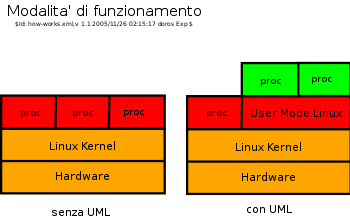
\includegraphics[width=7cm]{how-works.png}
  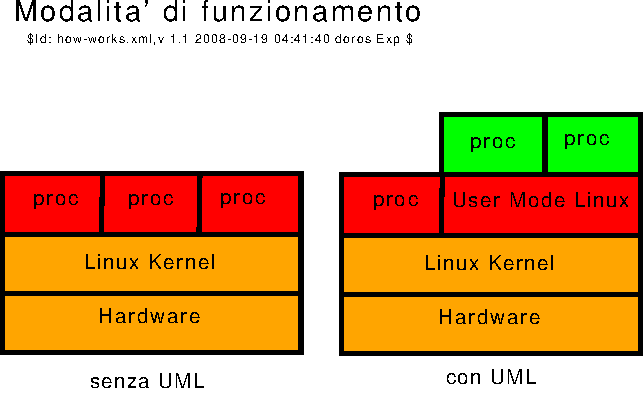
\includegraphics[width=0.6\textwidth]{how-works.pdf}
  \end{center}
}
\subsection{QEMU}
\frame{
  \frametitle{QEMU processor emulator}
  \begin{block}{http://fabrice.bellard.free.fr/qemu/}
  Il progetto \`{e} ideato e coordinato dal francese
  Fabrice Bellard. \`{E} un emulatore multipiattaforma che
  permette di eseguire del codice Linux compilato per una
  particolare CPU su di un processore x86: per esempio
  codice SPARC o ARM.\\
  Per avere una maggire velocit\`{a} deve essere compilato
  anche il modulo acceleratore kqemu.
  \end{block}
}
\subsection{Applicazioni}
\frame{
  \frametitle{Applicazioni}
  I contesti in cui si utilizza la virtualizzazione di un intero sistema
  operativo sono ad esempio:

  \begin{itemize}
    \item Ambiente di testing di nuovo software
    \item Ambiente di simulazione di protocolli di rete
    \item Costruzione di Honeynet virtuali
    \item Costruzione di Virtual Host per Hosting Service
  \end{itemize}
}
\frame{
  \label{test (1)}
  \frametitle{UML - Ambiente di testing di nuovo software (1)}
  Il progetto OpenSWAN (IPsec per Linux):
  \begin{itemize}
    \item si basa su righe di codice
  estremamente complicate per la comunicazione in rete
    \item cifra tutto il traffico di rete
    \item Utilizza un sistema
  di chiavi dinamico che rende praticamente impossibile ad un osservatore
  di capire cosa viene trasmesso
    \item occorrono circa 6
  sistemi per testare completamente il codice prodotto e quindi \`{e}
  impossibile o troppo costoso tenere un tale sistema dispobile
  solo per questo scopo
  \end{itemize}
}
\frame{
  \label{test (2)}
  \frametitle{UML - Ambiente per testing di nuovo software (2)}
  Il progetto BorpLAN (http://sourceforge.net/projects/borplan):
  \begin{itemize}
    \item si tratta di una applicazione ``web based'' realizzata
  come stage estivo A.S. 2005
  da Simone Veronese ex studente dell'ITIS ``C.Zuccante'' di Mestre (VE) e
  finanziata dalla Cassa di Risparmio di Venezia. Lo scopo
  della applicazione \`{e} costruire un sistema di controllo capillare
  degli accessi alla rete scolastica tramite l'uso di un browser e
  di packet filter.
    \item 
  per testare completamente il codice prodotto 
  occorrono almeno 2 router, 2 pc client e un web server
  e quindi \`{e}
  difficile e costoso mettere a disposizione una tale struttura. Inoltre
  nel caso di bugs il sistema deve risultare pronto per l'accettazione
  e la verifica del bug stesso e per la successiva risoluzione.
  \end{itemize}
}
\frame{
  \label{simu}
  \frametitle{Ambiente di sperimentazione di protocolli di rete}
  Il progetto UMTS/TIC corsi C1 e C2 (2003/2004 e 2006/2007) \`{e} un progetto del MIUR
  per la formazione del personale interno (ATA e docenti) sulla
  infrastruttura tecnologica.\\
  Si sono verificati alcuni problemi:
  \begin{itemize}
    \item mancanza di un laboratorio creato appositamente e sempre accessibile
    ai corsisti per effettuare le loro prove
    \item mancanza di un sufficiente numero di computer
    \item impossibilit\`{a} di effettuare le esercitazioni a casa
  \end{itemize}
}
\frame{
  \frametitle{Laboratorio di sistemi/informatica}
  Negli istituti tecnici a indirizzo informatica (ABACUS/Sirio)
  nell'ultimo anno di corso, a volte anche prima, si studiano
  le reti e le applicazioni web. Per l'assimilizione effettiva
  da parte degli studenti \`{e} opportuno:
  \begin{itemize}
    \item mettere a disposizione \textbf{per ogni studente} un gruppo di sistemi
          da configurare e amministrare
    \item avere lo stesso sistema \textbf{a casa}
  \end{itemize}
}
\frame{
  \frametitle{Playgroud per sperimentazione 3GPP}
  \begin{itemize}
  \item Playgroud \`{e} inteso come tecnologia per ambienti di
  test dove si pu\`{o} giocare ("play") con le ultime
  novit\`{a} tecnologiche.
  \item 3GPP ossia Third Generation Partnership Project \`{e} un accordo di
  collaborazione, formalizzato nel dicembre 1998, fra enti che si occupano di
  standardizzare sistemi di telecomunicazione in diverse parti del mondo (da
  Wikipedia). In tale ambienti si sperimenta l'IPv6 mobile e il sistema
  IP Multimedia System (IMS).
  \end{itemize}
}
\frame{
  \frametitle{Costruzione di Honeynet (vasi di miele)}
  Gli Honeynet sono dei sistemi installati sulle reti e servono per attirare
  eventuali intrusi e per studiare le loro mosse.
  Queste reti
  di sistemi sono altamente controllate e quando uno dei sistemi
  \`{e} attaccato esso cattura tutta l'attivit\`{a} dell'intruso.
  Un articolo che spiega come costruirli \`{e}:
  \href{http://www.honeynet.org/papers/virtual/}{``Know Your Enemy: Defining Virtual Honeynets''}
  tradotti in italiano in una serie di tre articoli(
  \href{http://www.honeynet.org/papers/trans/nemico.html}{1},
  \href{http://www.honeynet.org/papers/trans/nemico2.html}{2},
  \href{http://www.honeynet.org/papers/trans/nemico3.html}{3})
}
\frame{
  \frametitle{Costruzione di Virtual Host per Hosting Service}
  La vendita di servizi di hosting \`{e} un mercato in forte crescita
  e spesso chi li utilizza desidera passare dalla soluzione
  di delega della gestione dei propri servizi al pieno possesso
  degli stessi per ottenere pi\`{u} flessibilit\`{a}.
  La soluzione pi\`{u} vantaggiosa \`{e} sicuramente l'acquisto
  di un sistema virtuale.
}





\section{Netkit}
\frame{
  \frametitle{Cos'\`{e} Netkit - http://www.netkit.org}
    Netkit \`{e} il risultato del lavoro di alcune persone del
    Networks Research Group dell'Universit\`{a} di Roma 3 e
    del Linux User Group LUG Roma 3. Il software \`{e} composto da:
  \begin{itemize}
    \item Un insieme predefinito di comandi per il setup di
          macchine virtuali
    \item Un filesystem con preinstallato il software
          necessario per le sperimentazioni
    \item Un kernel UML linux
  \end{itemize}
}
\subsection{Linee guida}
\frame{
  \frametitle{Linee guida}
  Netkit \`{e} stato concepito come un ambiente a basso costo per
  esperimenti di rete. All'interno del suo ambiente possono essere
  ``creati'' e interconessi dei completi router, switch e host. Tali
  apparati sono virtuali ma possono operare con molte delle
  caratteristiche possedute da quelli reali.
}
\frame{
  \frametitle{Considerazioni generali}
  \begin{itemize}
    \item Basato su User Mode Linux
    \item Ogni apparato di rete \`{e} una linux box
    \item Linux supporta quasi tutti i protocolli di rete
          e pu\`{o} essere configurato come bridge/switch o
          come router
  \end{itemize}
}
\frame{
  \frametitle{Struttura}
  \begin{itemize}
    \item Le varie istanze che simulano gli apparati di rete
          sono create all'interno dello stesso host
    \item Le varie istanze sono interconnesse in domini di
          collisione (hub/switch)
    \item Il ruoli dei nodi sono configurabili
  \end{itemize}
}
\subsection{Esperienze riproducibili}
\frame{
  \frametitle{Esperienze riproducibili}
  \begin{itemize}
    \item Esperienze base: rete minimale con due host, tabelle di routing,
          protocollo ARP, protocollo RIP.
    \item Esperienze applicative: configurazione di DNS e Mail server.
    \item Esperienze avanzate: esperienze su switch e STP.
    \item Esperienze su routing interdomio (bgp): routing tra Autonomous
          System.
  \end{itemize}
}
\subsection{VisualNetkit}
\frame{
  \frametitle{Visual Netkit}
  \begin{itemize}
    \item http://code.google.com/p/visual-netkit/
    \item \`{E} un ambiente grafico scritto in C++ e Qt4
          che permette di configurare un laboratorio Netkit
          in modo semplice ed intuitivo.
    \item Alla base del progetto la sua archittettura a plugin
          che permette di abilitare funzionalit\`{a} o
          servizi dei nodi della rete in funzione delle
          necessit\`{a} degli utenti.
    \item 
\includegraphics[width=3mm]{youtube.png}
          \href{http://http://www.youtube.com/watch?v=OU7iblJ4mI8}{ YouTube Video }
  \end{itemize}
}




\section{Netkit4TIC}
\frame{
  \frametitle{Netkit4TIC - http://www.tic.fdns.net/tic/html/lab.html}
  Questo progetto \`{e} nato nel 2003 dalla necessit\`{a} nei
  corsi UMTS/TIC C2 di un laboratorio
  di sperimentazione ``permanente''.\\
  Le aree di interesse, intersecate tra loro, si possono
  dividere in:
  \begin{itemize}
    \item problematiche di rete: lo stack TCP/IP e la
          progettazione in generale di reti
    \item configurazione servizi: Web, DNS, 
          directory services, file share, Kerberos, Terminal Server
    \item problematiche sulla sicurezza: cifratura,
          certificati elettronici, VPN
  \end{itemize}
}
\subsection{Struttura}
\frame{
  \frametitle{Struttura}
  \`{E} composto da due parti:
  \begin{enumerate}
    \item Live-DVD: \`{e} una distribuzione GNU/Linux in grado di
          ``eseguire'' le esperienze senza bisogno di installazione. Contiene:
    \begin{itemize}
      \item una versione di Knoppix elaborata per ottenere migliori
            prestazioni con UML.
      \item un kernel UML e un filesystem con preinstallato una parte
            della distribuzione GNU/Linux Debian Lenny
      \item un kernel UML e un filesystem con la distribuzione LEAF/Bering con
            librerie uClibc per sistemi embedded.
      \item una versione leggermente personalizzata di Netkit
    \end{itemize}
    \item Internet: dal sito
          \href{http://www.tic.fdns.net/tic/html/lab.html}{http://www.tic.fdns.net/tic/html/lab.html}
          sono scaricabili le esperienze virtuali (qualche KiB) in formato archivio compresso (tgz).
  \end{enumerate}
}
\subsection{Esperienze riproducibili}
\frame{
  \frametitle{lo stack TCP/IP e la progettazione di reti}
  \begin{block}{Esperienze riproducibili}
  \begin{itemize}
    \item bridge, Bridge+STP, VLAN, proxyARP
    \item tabella di routing (statica), protocollo OSPF, Controllo LAB
    \item Qualit\`{a} del Servizio (QoS)
    \item Esercizi: NetPractice
  \end{itemize}
  \end{block}
}
\frame{
  \frametitle{Web, DNS, directory services, Kerberos, cluster HA, file share, LTSP}
  \begin{block}{Esperienze riproducibili}
  \begin{itemize}
    \item file sharing: Samba, Samba Enterprise e HA Samba
    \item directory service: OpenLDAP
    \item Kerberos V e Single Sign On
    \item HA-Cluster, AFS, XFS
    \item Terminal Server
    \item Monitoraggio reti via SNMP
  \end{itemize}
  \end{block}
}
\frame{
  \frametitle{Sicurezza}
  \begin{block}{Esperienze riproducibili}
  \begin{itemize}
    \item Firewall
    \begin{itemize}
       \item a singola area interna
       \item con area interna e area smilitarizzata (DMZ)
       \item con due are perimetrali e backbone interno
    \end{itemize}
    \item PKI: OpenCA una infrastruttura Open Source 
    \item Protocolli SSH e SSL
    \item VPN
    \item Sistemi di rilevazione intrusioni (NIDS)
  \end{itemize}
  \end{block}
}
\subsection{La nuova release v3.0}
\frame{
  \frametitle{Novit\`{a} della versione 3.0 (
     
\includegraphics[width=3mm]{youtube.png}
          \href{http://www.youtube.com/watch?v=NjRCFdYqA-s}{ YouTube Video) }}
  \begin{block}{Host}
  \begin{itemize}
    \item Visual Netkit
  \end{itemize}
  \end{block}
  \begin{block}{Guest Kernels}
  \begin{itemize}
    \item Linux 2.6.22 UML di Netkit
    \item Linux 2.6.26 UML di Debian Lenny (DFSG)
  \end{itemize}
  \end{block}
  \begin{block}{Guest Filesystem}
  \begin{itemize}
    \item nodo Debian Lenny di 2GiB (occupato al 51\%)
  \end{itemize}
  \end{block}
}
\frame{
  \frametitle{selezione nodo Lenny}
  \begin{block}{v-command}
  \begin{itemize}
    \item selezione del kernel:\\
        -k \$NETKIT\_HOME/kernel/lenny
  \end{itemize}
  \end{block}
  \begin{block}{l-command}
  \begin{itemize}
    \item selezione del kernel:\\
        vm[k]=\$NETKIT\_HOME/kernel/lenny
  \end{itemize}
  \end{block}
}
\frame{
  \frametitle{selezione nodo Bering}
  \begin{block}{v-command}
  \begin{itemize}
    \item selezione del kernel:\\
          -k \$NETKIT\_HOME/kernel/ub.krnl
    \item selezione del software da installare sul Bering:\\
          --append=LRP=root,config,etc, ... ,customvm
  \end{itemize}
  \end{block}
  \begin{block}{l-command}
  \begin{itemize}
    \item selezione del kernel:\\
          vm[k]=\$NETKIT\_HOME/kernel/ub.krnl
    \item selezione del software da installare sul Bering:\\
          vm[append]=LRP=root,config,etc, ... ,customvm
  \end{itemize}
  \end{block}
}
\frame{
  \frametitle{aggiunta connessione di rete "reale"}
  \begin{block}{parametri}
  \begin{itemize}
    \item default netkit
    \item --append=``ethX=tuntap,tapY''
  \end{itemize}
  \end{block}
}
\subsection{Direzione futura}
\frame{
  \frametitle{Nella prossima versione 4.0}
  \begin{block}{Host}
  \begin{itemize}
    \item Utilizzazione di un pi\`{u} recente Knoppix (5.3.1 o 6.0) e
          con patch SKAS3 o meglio ancora SKAS4
  \end{itemize}
  \end{block}
  \begin{block}{Guest}
  \begin{itemize}
    \item abbandono della distribuzione LEAF/Bering sostituita
          in toto dalla nuova Debian Lenny in grado oramai
          di girare sulle box di tipo WRAP/ALIX.
  \end{itemize}
  \end{block}
}


\section*{Sommario}

\frame{
  \frametitle{Sommario}

  \begin{block}{Riassunto}
  \begin{itemize}
  \item
    Lo studio e la progettazione di reti e di servizi di rete \`{e} un
    elemento essenziale del nostro futuro.
  \item
    La modalit\`{a} dell'apprendimento virtuale \`{e} in grande
    espansione.
  \item
    Esiste una via economica e valida: Netkit4TIC
  \end{itemize}
  \end{block}{}

  \begin{block}{Problematiche  aperte}
    \begin{itemize}
    \item
      Adozione limitata a: Mestre, Padova, Vicenza, Firenze, Palermo e Messina
    \item
      Costruzione di una comunity per la costruzione, collezione
      e condivisione di esperienze virtuali
    \end{itemize}
  \end{block}


}

%\frame{}   % to enforce entries in the table of contents

\end{document}
